\documentclass[10pt,aspectratio=169]{beamer}

\usetheme{Madrid}
\usepackage[T1]{fontenc}
\usepackage[utf8]{inputenc}
\usepackage{amsmath,amssymb}
\usepackage{booktabs}
\usepackage{graphicx}
\usepackage{xcolor}

\definecolor{accent}{HTML}{2563EB}
\definecolor{accent2}{HTML}{DC2626}
\definecolor{accent3}{HTML}{059669}
\definecolor{good}{HTML}{059669}
\definecolor{bad}{HTML}{DC2626}

\setbeamercolor{frametitle}{bg=accent,fg=white}
\setbeamertemplate{itemize item}{\textcolor{accent}{$\bullet$}}
\setbeamertemplate{navigation symbols}{}
\setbeamertemplate{footline}[frame number]

\title{Competing Risks: Prepayment vs.\ Default}
\subtitle{Part E(i) --- Mortgage Survival Analysis}
\author{Yueqi Lin}
\institute{MTH 9877 --- Baruch College, Spring 2026}
\date{May 13, 2026}

% =========================================================================
\begin{document}

% ---- Title ---------------------------------------------------------------
\begin{frame}[plain]
    \titlepage
\end{frame}

% ---- 1. Vintage defines the risk regime ----------------------------------
\begin{frame}{Vintage era --- not FICO or LTV --- is the dominant risk driver.}
    \begin{center}
        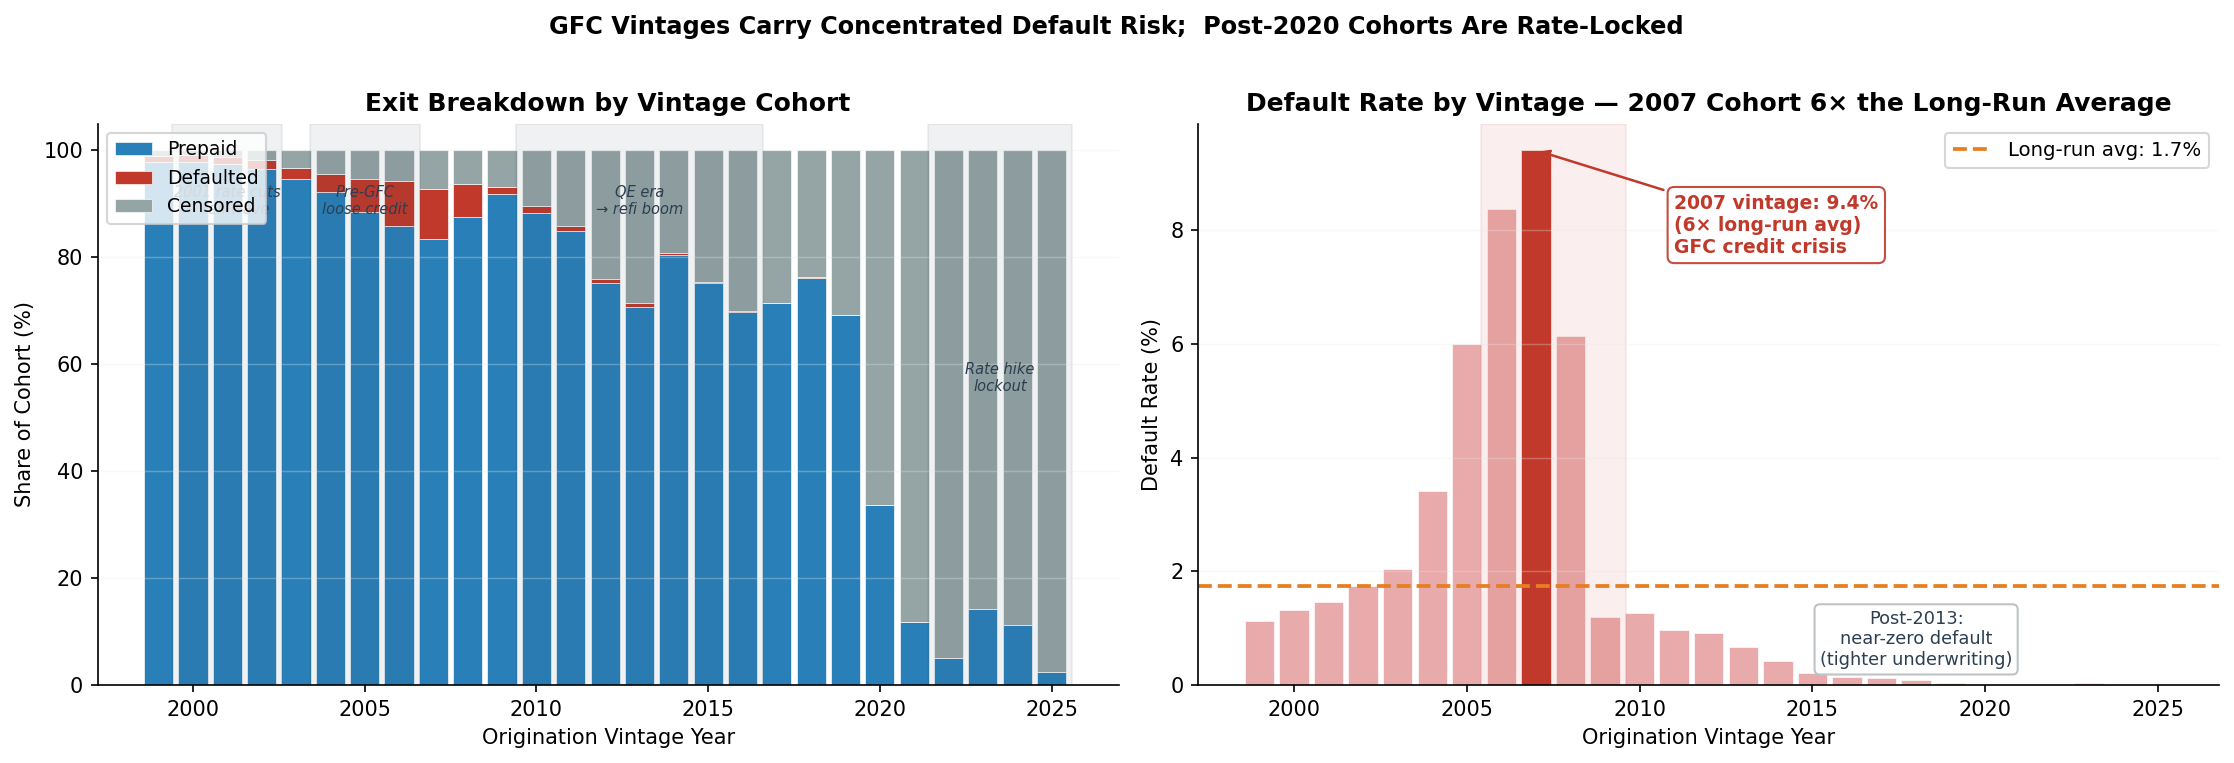
\includegraphics[width=0.92\linewidth]{processed/E1_eda_vintage}
    \end{center}
\end{frame}

% ---- 2. The two-cause problem --------------------------------------------
\begin{frame}{Two competing fates, two different borrower stories.}
    \begin{center}
        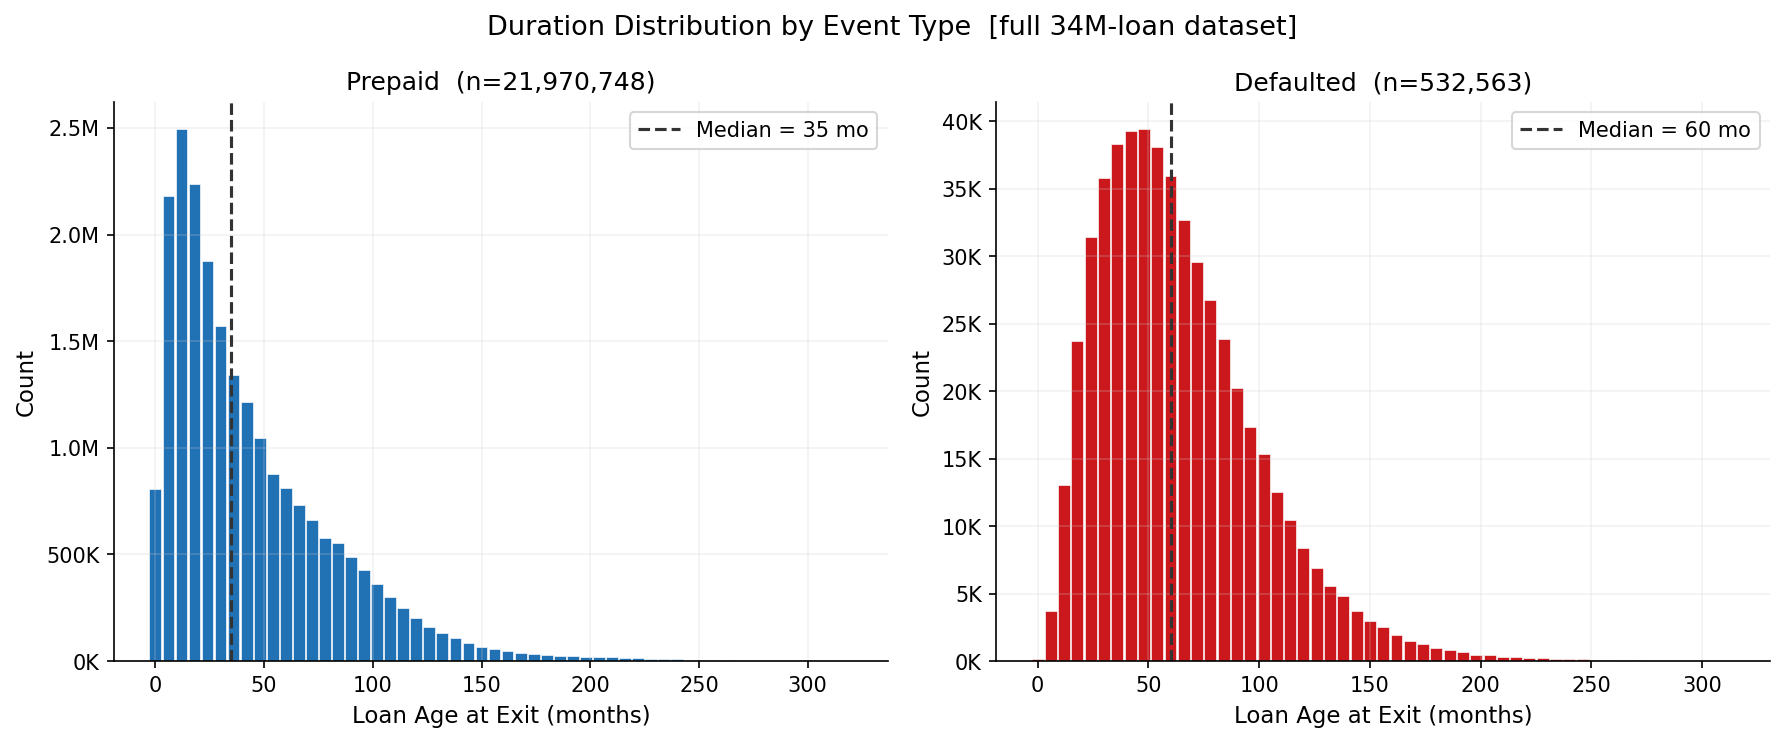
\includegraphics[width=0.92\linewidth]{processed/E1_eda_duration}
    \end{center}
\end{frame}

% ---- 3. KM vs AJ contrast ---------------------------------------------------
\begin{frame}{Two estimators, two different treatments of competing events.}
    \begin{columns}[T,onlytextwidth]
        \column{0.48\textwidth}
        \begin{block}{Kaplan--Meier}
        \[
            \hat{F}^{(k)}_{\mathrm{KM}}(t)
            = 1 - \prod_{t_j \le t}\!\left(1 - \frac{d_{j}^{(k)}}{n_j^{\mathrm{KM}}}\right)
        \]
        \vspace{0.1em}
        \small
        \begin{tabular}{@{}ll@{}}
            $d_j^{(k)}$ & cause-$k$ exits at $t_j$ \\[2pt]
            $n_j^{\mathrm{KM}}$ & risk set excluding competing-event loans \\[2pt]
        \end{tabular}
        \end{block}

        \column{0.48\textwidth}
        \begin{block}{Aalen--Johansen}
        \[
            \hat{F}_k(t) = \sum_{t_j \le t} \hat{S}(t_j^{-})\cdot \frac{d_{kj}}{n_j}
        \]
        \vspace{0.1em}
        \small
        \begin{tabular}{@{}ll@{}}
            $d_{kj}$        & cause-$k$ exits at $t_j$ \\[2pt]
            $n_j$           & risk set including all exits \\[2pt]
            $\hat{S}(t_j^-)$ & overall survival just before $t_j$ \\[2pt]
        \end{tabular}
        \end{block}
    \end{columns}
    \vspace{0.6em}
    \begin{center}
        \small
        KM: competing exits censored $\Rightarrow$ denominator too small $\Rightarrow$ each increment inflated.\\[3pt]
        AJ: $\hat{S}(t_j^-)$ shrinks with every exit $\Rightarrow$ $\hat{F}^{(\mathrm{pre})} + \hat{F}^{(\mathrm{def})} + \hat{S} = 1$ always.
    \end{center}
\end{frame}

% ---- 4. AJ CIF formula + result ------------------------------------------
\begin{frame}{The Aalen--Johansen estimator gives the only coherent probability partition.}
    \begin{columns}[c,onlytextwidth]
        \column{0.64\textwidth}
        \begin{center}
            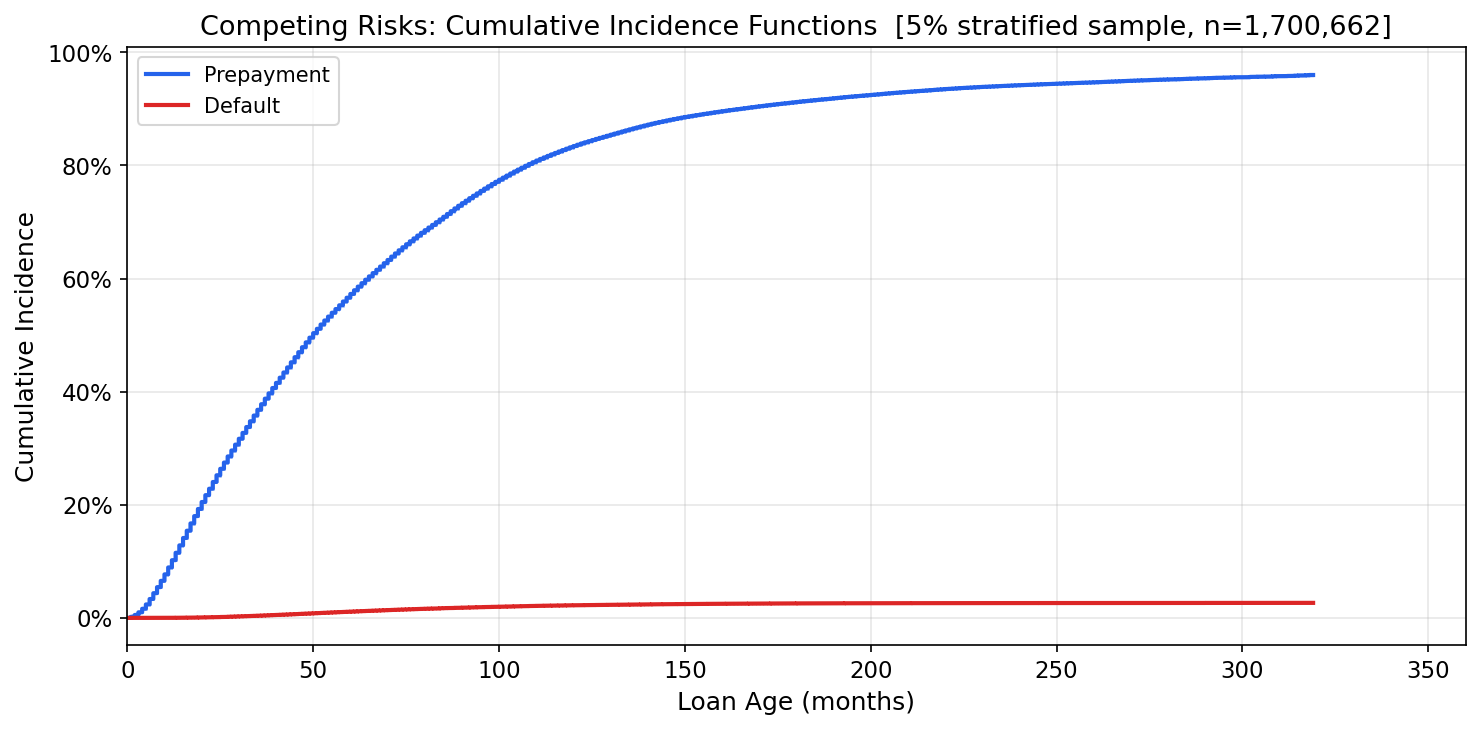
\includegraphics[width=\linewidth]{processed/E1_competing_risks_cif}
        \end{center}

        \column{0.34\textwidth}
        \begin{center}
        \vspace{1em}
        \small
        \textbf{Cumulative Incidence Function}\\[3pt]
        $F_k(t) = P(\text{exit by }t,\ \text{cause }k)$\\[10pt]
        \textbf{Aalen--Johansen CIF partition}\\[4pt]
        \begin{tabular}{lccc}
            \toprule
            & Prepaid & Default & Active \\
            \midrule
            5 yr  & 61.4\% & 1.1\% & 37.6\% \\
            10 yr & 83.3\% & 2.2\% & 14.5\% \\
            20 yr & 91.8\% & 3.1\% &  5.1\% \\
            \bottomrule
        \end{tabular}
        \end{center}
    \end{columns}
\end{frame}

% ---- 4. KM is wrong --------------------------------------------------------
\begin{frame}{KM overstates prepayment probability because it ignores competing defaults.}
    \begin{center}
        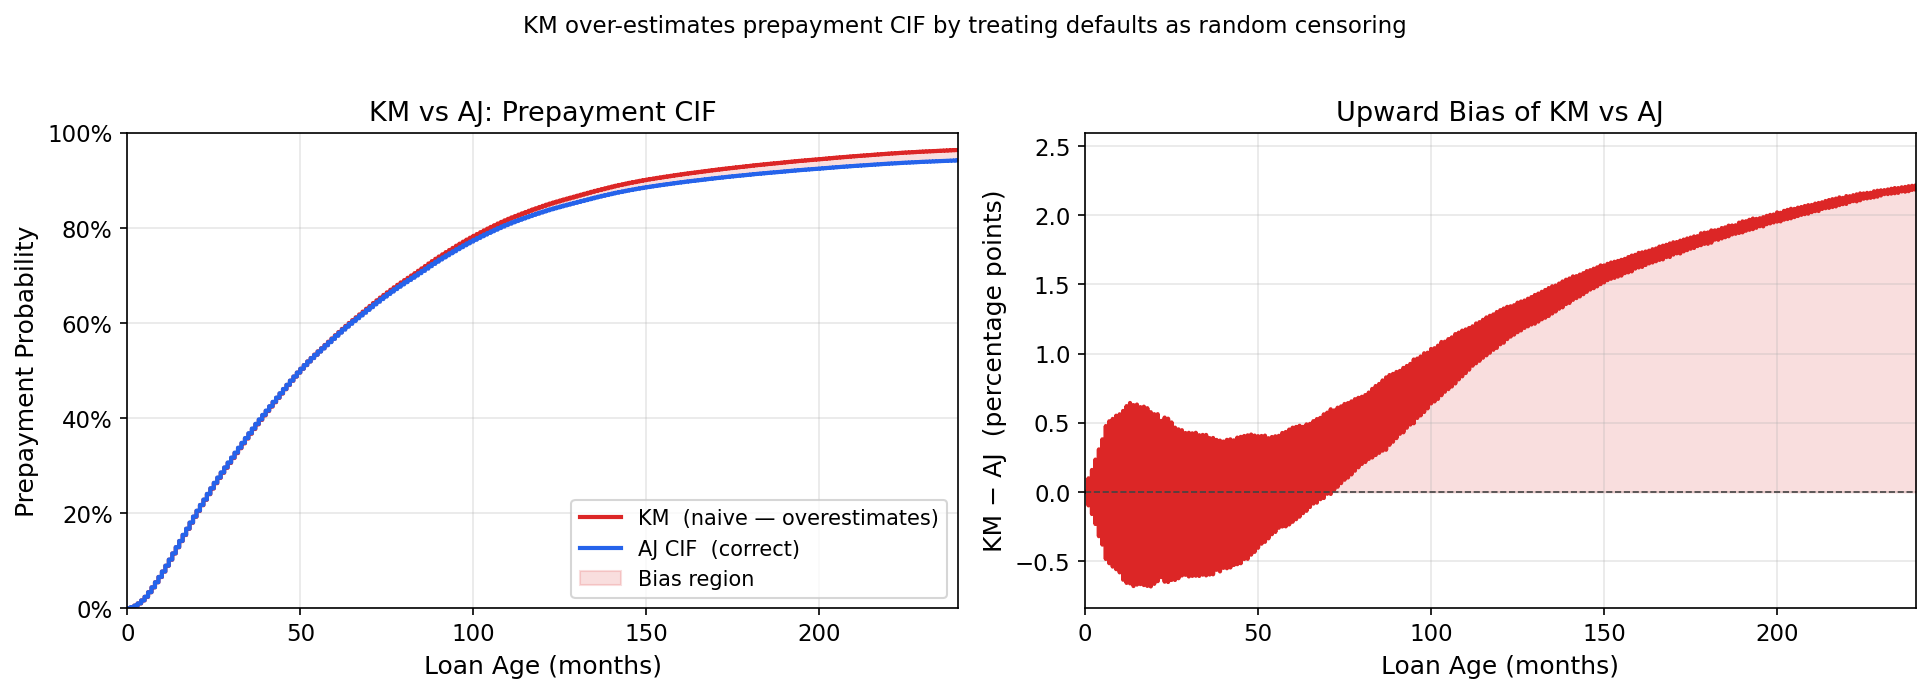
\includegraphics[width=0.82\linewidth]{processed/E1_km_vs_aj_bias}
    \end{center}
    \vspace{-0.3em}
    \begin{center}
        \small
        \textbf{KM overstatement of prepayment probability}\\[4pt]
        \begin{tabular}{lccc}
            \toprule
            Horizon & $\hat{F}_{\mathrm{KM}}$ & $\hat{F}_{\mathrm{AJ}}$ & Bias \\
            \midrule
            5 yr  & 61.9\% & 61.4\% & $+$0.45 pp \\
            10 yr & 84.6\% & 83.3\% & $+$1.31 pp \\
            20 yr & 93.4\% & 91.8\% & $+$2.23 pp \\
            \bottomrule
        \end{tabular}
    \end{center}
\end{frame}

% ---- 5. Stratified CIF ---------------------------------------------------
\begin{frame}{FICO separates default 6$\times$; LTV separates default 2$\times$ --- neither separates prepayment.}
    \begin{center}
        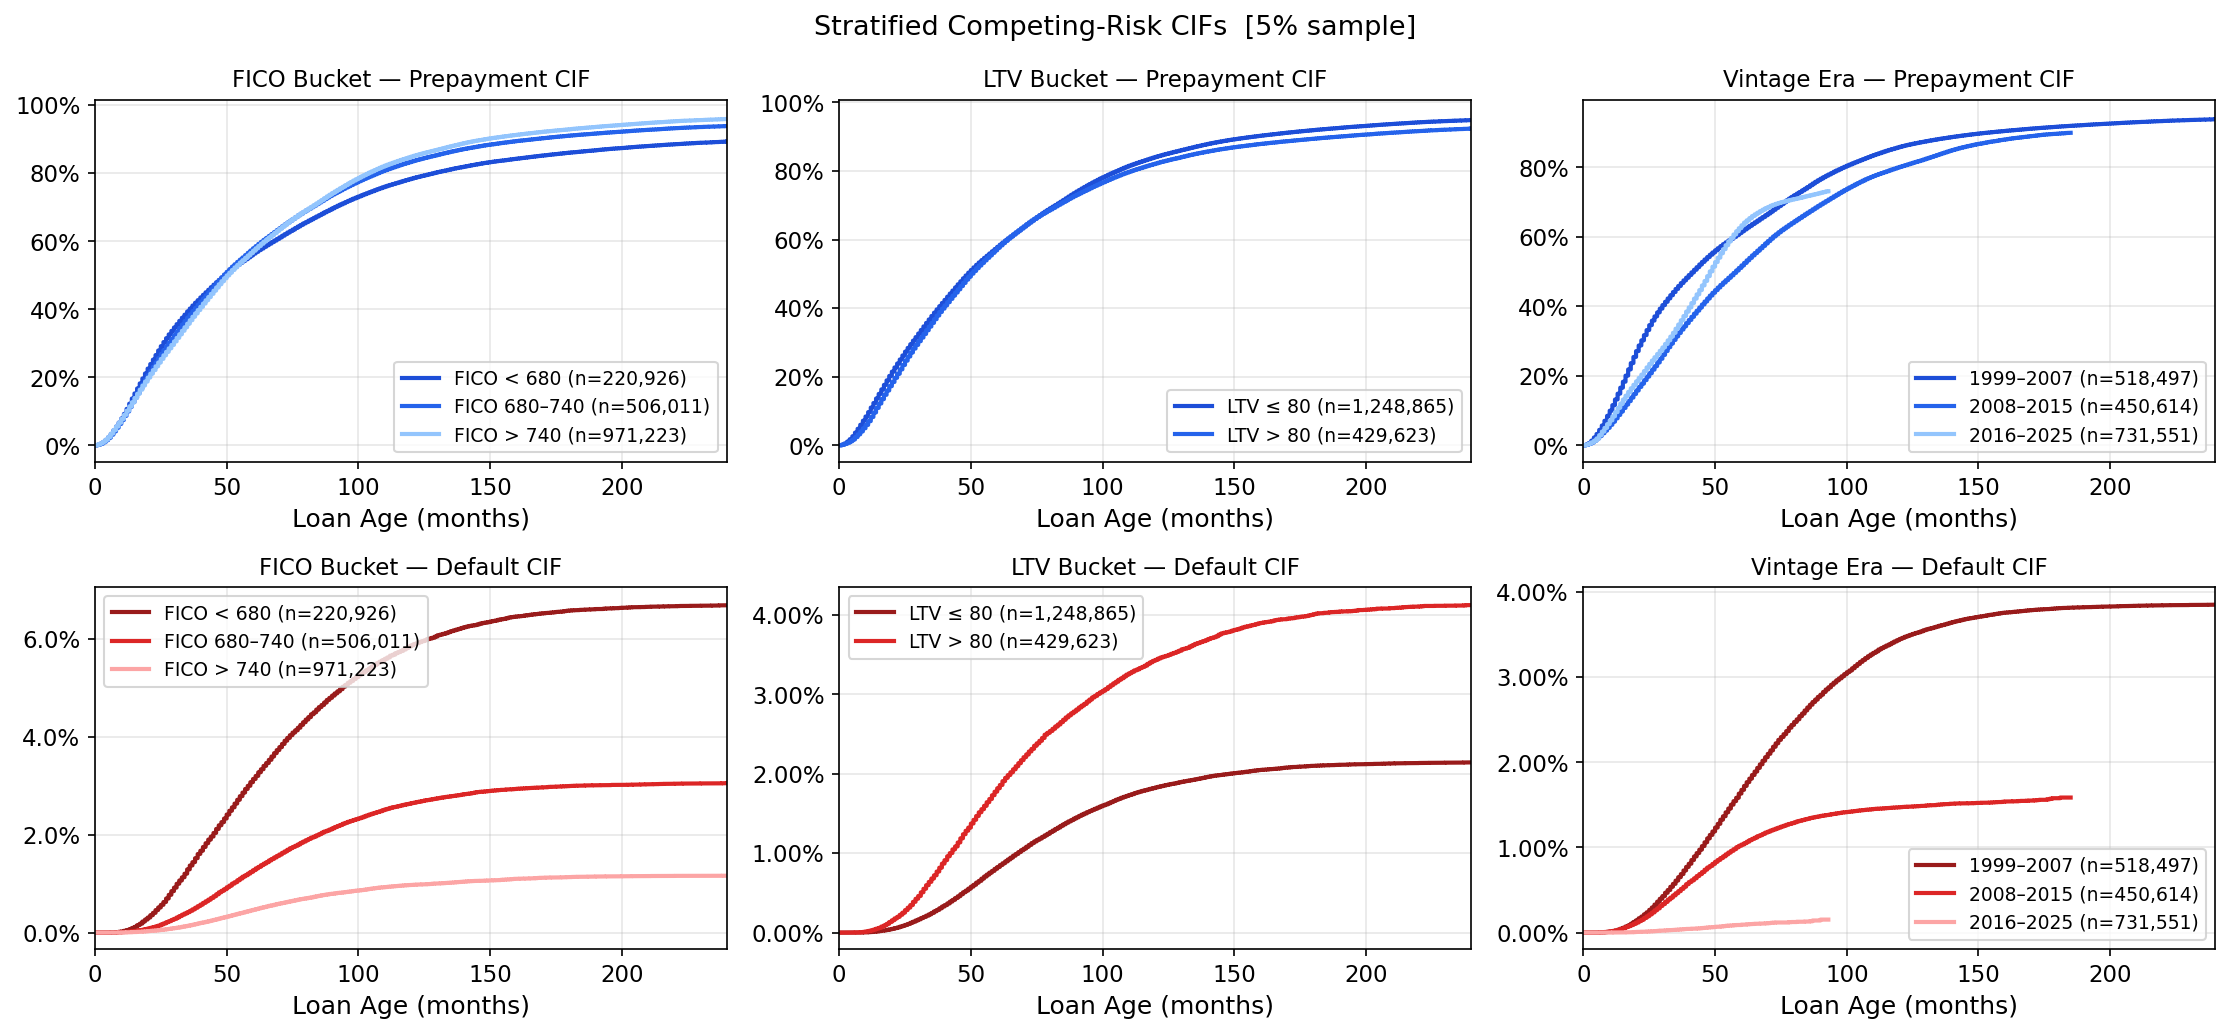
\includegraphics[height=0.78\textheight,keepaspectratio]{processed/E1_stratified_cif}
    \end{center}
\end{frame}

% ---- 6. Cause-specific Cox model -----------------------------------------
\begin{frame}{Cause-specific Cox: one separate hazard model per cause.}
    \begin{columns}[T,onlytextwidth]
        \column{0.54\textwidth}
        \begin{block}{Cause-Specific Cox}
        \[
            h_k(t \mid \mathbf{x}) = h_{0k}(t)\,\exp\!\bigl(\boldsymbol{\beta}_k^\top\mathbf{x}\bigr),
            \quad k \in \{\mathrm{pre},\,\mathrm{def}\}
        \]
        \[
            \ell(\boldsymbol{\beta}_k) = \sum_{i:\,E_i=k}
            \!\Biggl[
                \boldsymbol{\beta}_k^\top \mathbf{x}_i
                - \log\!\sum_{j\in\mathcal{R}(t_i)}
                e^{\boldsymbol{\beta}_k^\top\mathbf{x}_j}
            \Biggr]
        \]
        \end{block}
        \vspace{0.4em}
        \small
        $\mathcal{R}(t_i)$: all loans still active just before $t_i$.\\[3pt]
        Competing-cause exits are \textbf{censored} --- they leave
        $\mathcal{R}(t)$ without contributing to $\ell$.

        \column{0.42\textwidth}
        \small\vspace{0.4em}

        \normalsize\textbf{Additional features}\\[6pt]
        \small
        \textbf{Max Delinquency} --- months past due over loan life\\[6pt]
        \textbf{Ever 90+ DQ} --- binary flag for severe delinquency
    \end{columns}
\end{frame}

% ---- 7. CS-Cox forest plots ----------------------------------------------
\begin{frame}{Prepayment and default respond to opposite covariate effects.}
    \begin{center}
        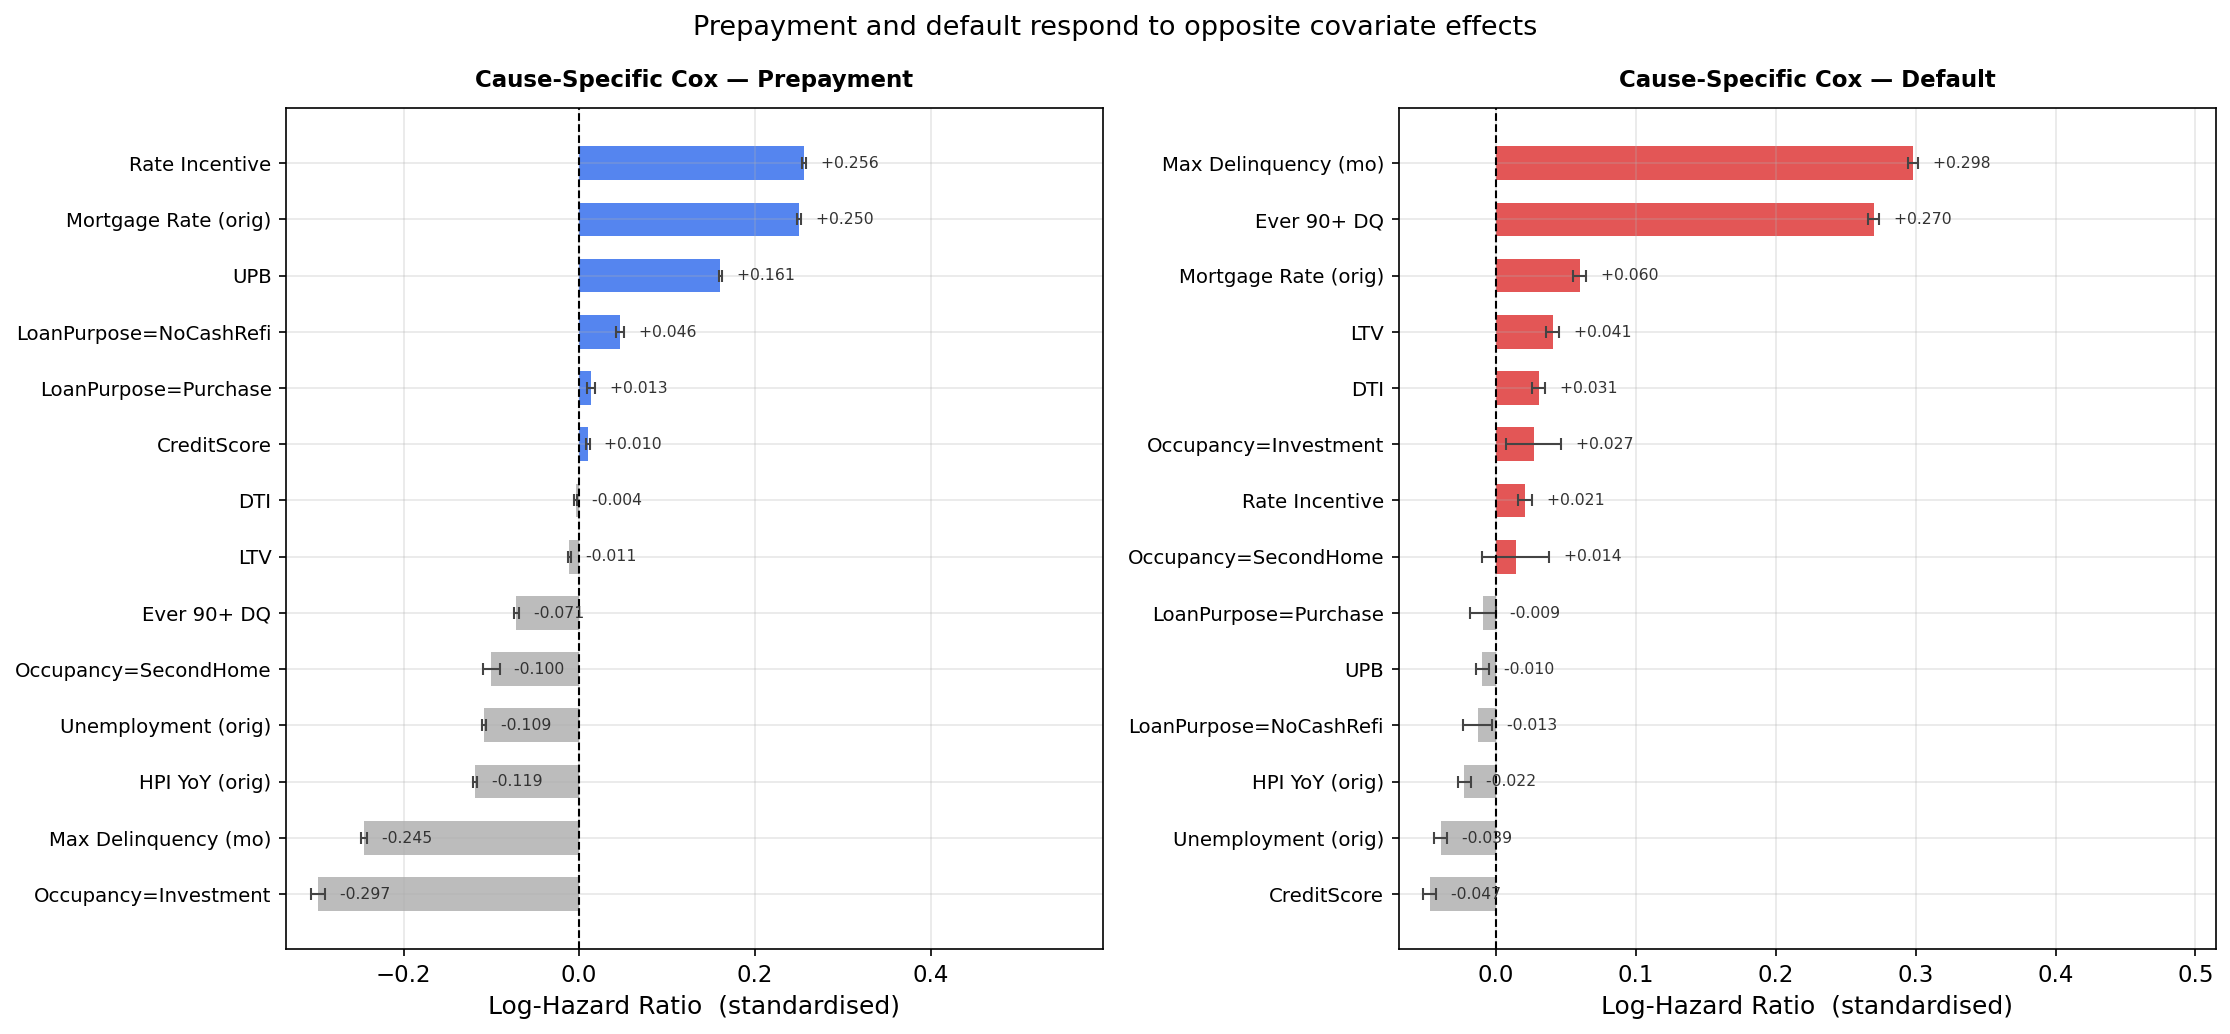
\includegraphics[width=\linewidth]{processed/E1_cause_specific_cox}
    \end{center}
\end{frame}

% ---- 7. Opposite signs table ---------------------------------------------
\begin{frame}{Four covariates flip sign --- a combined model cancels both signals.}
    \vspace{0.2em}
    \begin{center}
    \small
    \textbf{Naive Cox vs.\ cause-specific coefficients}\\[4pt]
    \begin{tabular}{lrrrp{2.6cm}}
        \toprule
        \textbf{Covariate} & \textbf{Naive $\hat\beta$} & \textbf{Prepay $\hat\beta$} & \textbf{Default $\hat\beta$} & \\
        \midrule
        Rate incentive   & $+0.253$ & \textcolor{good}{$+0.256$} & $+0.021$                   & (pure prepay) \\
        UPB              & $+0.161$ & \textcolor{good}{$+0.161$} & $-0.010$                   & (pure prepay) \\
        \midrule
        FICO             & $+0.016$ & \textcolor{good}{$+0.010$} & \textcolor{bad}{$-0.047$}  & \textbf{opposite} \\
        LTV              & $-0.007$ & \textcolor{bad}{$-0.011$}  & \textcolor{good}{$+0.041$} & \textbf{opposite} \\
        Max Delinquency  & $-0.123$ & \textcolor{bad}{$-0.245$}  & \textcolor{good}{$+0.298$} & \textbf{opposite} \\
        Ever 90+ DQ      & $-0.035$ & \textcolor{bad}{$-0.071$}  & \textcolor{good}{$+0.270$} & \textbf{opposite} \\
        \bottomrule
    \end{tabular}
    \end{center}
    \vspace{0.3em}
    \begin{center}
        \small
        Each extra month delinquent raises default hazard by $35\%$ and cuts prepayment hazard by $22\%$
        --- yet the naive coefficient ($-0.123$) conceals both, collapsing a $+0.543$ spread to near zero.
    \end{center}
\end{frame}

% ---- 8. Key Takeaways ----------------------------------------------------
\begin{frame}{Key Takeaways}
    \begin{enumerate}\itemsep8pt
        \item \textbf{Default and prepayment are competing risks}\\
              \small A naive Cox model is biased and conflates two economically opposite processes.

        \item \textbf{Kaplan--Meier overstates prepayment probability by up to $+$2.2\,pp}\\
              \small It ignores the competing cause absorbing risk; Aalen--Johansen is required.

        \item \textbf{CIF curves reveal large cohort-level variation}\\
              \small The 2007 cohort's default CIF is $6\times$ the long-run average; post-2020 prepayment CIF is nearly flat due to rate lock-in.

        \item \textbf{FICO drives default; rate incentive drives prepayment}\\
              \small Each feature is essentially invisible to the other cause --- the two risks operate through separate channels.

        \item \textbf{Fine--Gray and cause-specific Cox give similar results here}\\
              \small The gap opens when default and prepayment are strongly correlated --- crisis vintages or high-risk borrowers.
    \end{enumerate}
\end{frame}

% ---- Thank you ------------------------------------------------------------
\begin{frame}[plain]
    \vspace*{2em}
    \begin{center}
        {\Huge \textbf{Thank you}}\\[1.5em]
        {\Large Questions?}\\[2.5em]
        \small
        Fine \& Gray (1999) \textit{JASA} $\cdot$
        Aalen \& Johansen (1978) \textit{Scand.\ J.\ Stat.} $\cdot$
        Sadhwani et al.\ (2021) \textit{J.\ Fin.\ Econometrics}
    \end{center}
\end{frame}

\end{document}
